\documentclass[main.tex]{subfiles}

\begin{document}

\section{A2 Hybrid Mobile Application}

\subsection{Szenario}

Sie wollen objektorientiert ein hybrides Application Framework entwickeln, mit dem Sie einheitlich graphische Benutzerschnittstellen in Android und iOS steuern können. Sie benötigen die folgenden Klassen:

\begin{itemize}
    \item Eine generalisierte Klasse \lstinline|MobileElement| mit dem schreibgeschützten Attribut \lstinline|getTitle()| vom Datentyp String sowie den rückgabelosen Operationen \lstinline|render()| und \lstinline|register(MobileForm form)|.
    \item Eine generalisierte Klasse \lstinline|MobileForm| mit folgenden Klassenmitgliedern:
    \begin{itemize}
        \item Liste der enthaltenen mobilen Elemente vom Typ \lstinline|MobileElement|. Das Verhältnis ist eine Teile-Ganze-Beziehung.
        \item Operation \lstinline|addElement(string title)|: es wird ein neues mobiles Element mit dem angegebenen Titel erzeugt. Der Titel kann nur bei der Erzeugung festgelegt werden. Während der Erzeugung wird die zugehörige \lstinline|MobileForm| registriert.
        \item Operation \lstinline|render()|, die die gleichnamige Operation in allen enthaltenen mobilen Elementen aufruft.
    \end{itemize}
    \item Von \lstinline|MobileElement| und \lstinline|MobileForm| sollen keine Instanzen erzeugt werden können.
    \item Konkrete Elemente und konkrete Formen für Android und iOS, die erzeugt werden können. Die Betriebssysteme einer konkreten Form und den darin enthaltenen konkreten Elementen passen immer zusammen.
    \item Alle oben genannten Klassen sind im Paket \lstinline|mobileapplication.ui| enthalten. Aus Sicherheitsgründen sollen neue konkrete Elemente von außerhalb des Pakets nur über die Operation \lstinline|addElement| von \lstinline|MobileForm| erzeugt werden können.
    \item Die Klasse \lstinline|App| im Paket \lstinline|mobileapplication| mit den folgenden Eigenschaften:
    \begin{itemize}
        \item Attribut \lstinline|form| vom Datentyp \lstinline|MobileForm|.
        \item Private Operation \lstinline|getOS()|, die das aktuelle Betriebssystem als String zurückgibt. \\
        Mögliche Werte sind zurzeit »Android« und »iOS«.
        \item Private Operation \lstinline|initialize()|, die dem Attribut \lstinline|form| eine neue Instanz passend zum Betriebssystem zuweist.
        \item Operation \lstinline|execute()|, die \lstinline|initialize()| aufruft, drei neue Elemente der konkreten Form hinzufügt und anschließend alle Elemente rendert.
    \end{itemize}
\end{itemize}

\subsection{Aufgaben}
\begin{enumerate}
    \item Entwerfen Sie eine Lösung als Klassenverband. Nutzen Sie dafür das Entwurfsmuster Factory Method, wobei \lstinline|MobileForm| die Rolle von Creator und \lstinline|MobileElement| die Rolle von \lstinline|Product| übernehmen soll. Modellieren Sie den Klassenverband als UML-Klassendiagramm.
    \item Modellieren Sie die Abfolge der Aufrufe als UML-Sequenzdiagramm. Beginnen Sie mit der Operation \lstinline|execute()| der Klasse App als gefundene Nachricht. Nutzen Sie dabei die abstrakten und nicht die konkreten Klassen.
    \item Implementieren Sie den Rumpf der Lösung in Java.
\end{enumerate}

\subsection{Lösung 2}
\begin{figure}[h]
    \makebox[\textwidth][c]{
        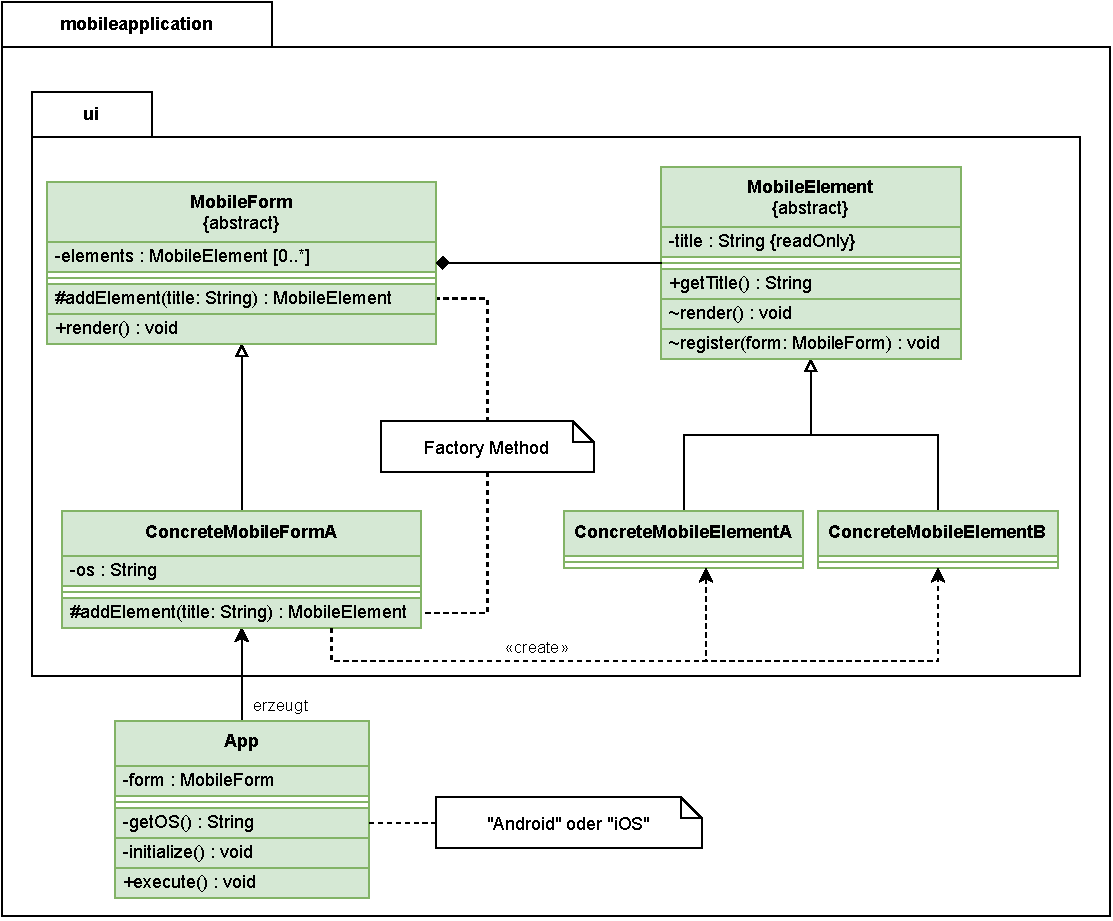
\includegraphics[width=1.2\linewidth]{A2-a.pdf}
    }
    \caption{Lösung der Aufgabe 2a}
    \label{fig:lgs2a}
\end{figure}

\begin{figure}[h]
    \makebox[\textwidth][c]{
        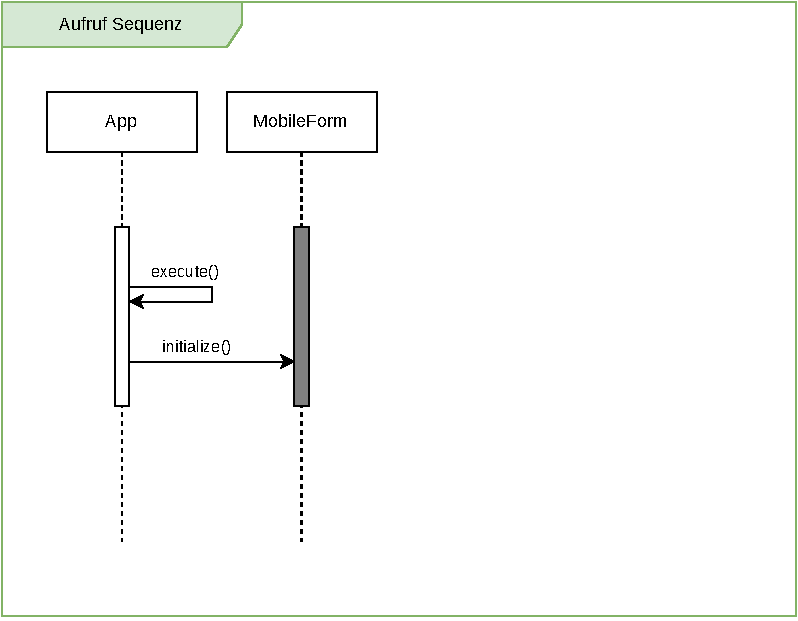
\includegraphics[width=0.4\linewidth]{A2-b.pdf}
    }
    \caption{Lösung der Aufgabe 2b}
    \label{fig:lgs2b}
\end{figure}

\end{document}
